\documentclass[a4paper,12pt]{extreport}

%====================== PACKAGES ======================
%%%%%%%%%%%%%%%%%%%%%%%%%%%%%%%%%%%%%%%%%
% Lachaise Assignment
% Structure Specification File
% Version 1.0 (26/6/2018)
%
% This template originates from:
% http://www.LaTeXTemplates.com
%
% Authors:
% Marion Lachaise & François Févotte
% Vel (vel@LaTeXTemplates.com)
%
% License:
% CC BY-NC-SA 3.0 (http://creativecommons.org/licenses/by-nc-sa/3.0/)
% 
%%%%%%%%%%%%%%%%%%%%%%%%%%%%%%%%%%%%%%%%%

%----------------------------------------------------------------------------------------
%	PACKAGES AND OTHER DOCUMENT CONFIGURATIONS
%----------------------------------------------------------------------------------------

\usepackage{amsmath,amsfonts,stmaryrd,amssymb} % Math packages

\usepackage{enumerate} % Custom item numbers for enumerations

\usepackage[ruled]{algorithm2e} % Algorithms

\usepackage[framemethod=tikz]{mdframed} % Allows defining custom boxed/framed environments

\usepackage{listings} % File listings, with syntax highlighting
\lstset{
	basicstyle=\ttfamily, % Typeset listings in monospace font
}

%----------------------------------------------------------------------------------------
%	DOCUMENT MARGINS
%----------------------------------------------------------------------------------------

\usepackage{geometry} % Required for adjusting page dimensions and margins

\geometry{
	paper=a4paper, % Paper size, change to letterpaper for US letter size
	top=2.5cm, % Top margin
	bottom=3cm, % Bottom margin
	left=2.5cm, % Left margin
	right=2.5cm, % Right margin
	headheight=14pt, % Header height
	footskip=1.5cm, % Space from the bottom margin to the baseline of the footer
	headsep=1.2cm, % Space from the top margin to the baseline of the header
	%showframe, % Uncomment to show how the type block is set on the page
}

%----------------------------------------------------------------------------------------
%	FONTS
%----------------------------------------------------------------------------------------

\usepackage[utf8]{inputenc} % Required for inputting international characters
\usepackage[T1]{fontenc} % Output font encoding for international characters

%\usepackage{XCharter} % Use the XCharter fonts

%----------------------------------------------------------------------------------------
%	COMMAND LINE ENVIRONMENT
%----------------------------------------------------------------------------------------

% Usage:
% \begin{commandline}
%	\begin{verbatim}
%		$ ls
%		
%		Applications	Desktop	...
%	\end{verbatim}
% \end{commandline}

\mdfdefinestyle{commandline}{
	leftmargin=10pt,
	rightmargin=10pt,
	innerleftmargin=15pt,
	middlelinecolor=black!50!white,
	middlelinewidth=2pt,
	frametitlerule=false,
	backgroundcolor=black!5!white,
	frametitle={Command Line},
	frametitlefont={\normalfont\sffamily\color{white}\hspace{-1em}},
	frametitlebackgroundcolor=black!50!white,
	nobreak,
}

% Define a custom environment for command-line snapshots
\newenvironment{commandline}{
	\medskip
	\begin{mdframed}[style=commandline]
}{
	\end{mdframed}
	\medskip
}

%----------------------------------------------------------------------------------------
%	FILE CONTENTS ENVIRONMENT
%----------------------------------------------------------------------------------------

% Usage:
% \begin{file}[optional filename, defaults to "File"]
%	File contents, for example, with a listings environment
% \end{file}

\mdfdefinestyle{file}{
	innertopmargin=1.6\baselineskip,
	innerbottommargin=0.8\baselineskip,
	topline=false, bottomline=false,
	leftline=false, rightline=false,
	leftmargin=2cm,
	rightmargin=2cm,
	singleextra={%
		\draw[fill=black!10!white](P)++(0,-1.2em)rectangle(P-|O);
		\node[anchor=north west]
		at(P-|O){\ttfamily\mdfilename};
		%
		\def\l{3em}
		\draw(O-|P)++(-\l,0)--++(\l,\l)--(P)--(P-|O)--(O)--cycle;
		\draw(O-|P)++(-\l,0)--++(0,\l)--++(\l,0);
	},
	nobreak,
}

% Define a custom environment for file contents
\newenvironment{file}[1][File]{ % Set the default filename to "File"
	\medskip
	\newcommand{\mdfilename}{#1}
	\begin{mdframed}[style=file]
}{
	\end{mdframed}
	\medskip
}

%----------------------------------------------------------------------------------------
%	NUMBERED QUESTIONS ENVIRONMENT
%----------------------------------------------------------------------------------------

% Usage:
% \begin{question}[optional title]
%	Question contents
% \end{question}

\mdfdefinestyle{question}{
	innertopmargin=1.2\baselineskip,
	innerbottommargin=0.8\baselineskip,
	roundcorner=5pt,
	nobreak,
	singleextra={%
		\draw(P-|O)node[xshift=1em,anchor=west,fill=white,draw,rounded corners=5pt]{%
		Question \theQuestion\questionTitle};
	},
}

\newcounter{Question} % Stores the current question number that gets iterated with each new question

% Define a custom environment for numbered questions
\newenvironment{question}[1][\unskip]{
	\bigskip
	\stepcounter{Question}
	\newcommand{\questionTitle}{~#1}
	\begin{mdframed}[style=question]
}{
	\end{mdframed}
	\medskip
}

%----------------------------------------------------------------------------------------
%	WARNING TEXT ENVIRONMENT
%----------------------------------------------------------------------------------------

% Usage:
% \begin{warn}[optional title, defaults to "Warning:"]
%	Contents
% \end{warn}

\mdfdefinestyle{warning}{
	topline=false, bottomline=false,
	leftline=false, rightline=false,
	nobreak,
	singleextra={%
		\draw(P-|O)++(-0.5em,0)node(tmp1){};
		\draw(P-|O)++(0.5em,0)node(tmp2){};
		\fill[black,rotate around={45:(P-|O)}](tmp1)rectangle(tmp2);
		\node at(P-|O){\color{white}\scriptsize\bf !};
		\draw[very thick](P-|O)++(0,-1em)--(O);%--(O-|P);
	}
}

% Define a custom environment for warning text
\newenvironment{warn}[1][Warning:]{ % Set the default warning to "Warning:"
	\medskip
	\begin{mdframed}[style=warning]
		\noindent{\textbf{#1}}
}{
	\end{mdframed}
}

%----------------------------------------------------------------------------------------
%	INFORMATION ENVIRONMENT
%----------------------------------------------------------------------------------------

% Usage:
% \begin{info}[optional title, defaults to "Info:"]
% 	contents
% 	\end{info}

\mdfdefinestyle{info}{%
	topline=false, bottomline=false,
	leftline=false, rightline=false,
	nobreak,
	singleextra={%
		\fill[black](P-|O)circle[radius=0.4em];
		\node at(P-|O){\color{white}\scriptsize\bf i};
		\draw[very thick](P-|O)++(0,-0.8em)--(O);%--(O-|P);
	}
}

% Define a custom environment for information
\newenvironment{info}[1][Info:]{ % Set the default title to "Info:"
	\medskip
	\begin{mdframed}[style=info]
		\noindent{\textbf{#1}}
}{
	\end{mdframed}
}
 % Include the file specifying the document structure and custom commands
\usepackage{graphicx}
\usepackage{gensymb}
\usepackage{float}
\usepackage[french]{babel}
\usepackage{comment}

%\usepackage[utf8x]{inputenc}
%pour les informations sur un document compilé en PDF et les liens externes / internes
\usepackage{hyperref}
%pour la mise en page des tableaux
%\usepackage{array}
%\usepackage{tabularx}
%pour utiliser \floatbarrier
%\usepackage{placeins}
%\usepackage{floatrow}
%espacement entre les lignes
%\usepackage{setspace}
%modifier la mise en page de l'abstract
\usepackage{abstract}
%police et mise en page (marges) du document
%\usepackage[T1]{fontenc}
%\usepackage[top=2cm, bottom=2cm, left=2cm, right=2cm]{geometry}



%====================== INFORMATION ET REGLES ======================

%rajouter les numérotation pour les \paragraphe et \subparagraphe
\setcounter{secnumdepth}{4}
\setcounter{tocdepth}{4}

\hypersetup{							% Information sur le document
pdfauthor = {Premier Auteur,
			Deuxième Auteur,
			Troisième Auteur,
    		Quatrième Auteur},			% Auteurs
pdftitle = {Nom du Projet -
			Sujet du Projet},			% Titre du document
pdfsubject = {Intern Report},		% Sujet
pdfkeywords = {Tag1, Tag2, Tag3, ...},	% Mots-clefs
pdfstartview={FitH}}					% ajuste la page à la largueur de l'écran
%pdfcreator = {MikTeX},% Logiciel qui a crée le document
%pdfproducer = {}} % Société avec produit le logiciel

%======================== DEBUT DU DOCUMENT ========================

\begin{document}

%régler l'espacement entre les lignes
\newcommand{\HRule}{\rule{\linewidth}{0.5mm}}

%page de garde
\begin{titlepage}
\begin{center}

% Upper part of the page. The '~' is needed because only works if a paragraph has started.

\includegraphics[width=0.15\textwidth]{./images/logo-ensea.png}~\\[1cm]

\textsc{\Large  Ecole nationale supérieure de l'électronique et de ses applications}\\[0.5cm]

% Title
\HRule \\[0.4cm]

{\huge \bfseries RAPPORT PLT\\
Réalisation d'un T-RPG type Disgaea   \\[0.4cm] }

\HRule \\[1.5cm]

% Author and supervisor
\begin{minipage}{0.4\textwidth}
\begin{flushleft} \large
\emph{Authors:}\\
Benjamin \textsc{Anslot}\\
Mathieu \textsc{Hadjadji}
\end{flushleft}
\end{minipage}
\begin{minipage}{0.4\textwidth}
\begin{flushright} \large


\emph{Années:} \\
2019 - 2020 \\
OPTION IS \\
\end{flushright}
\end{minipage}

\vfill

% Bottom of the page
{\large \today}

\end{center}
\end{titlepage}

%page blanche
\newpage
~
%ne pas numéroter cette page
\thispagestyle{empty}
\newpage

% \renewcommand{\abstractnamefont}{\normalfont\Large\bfseries}
%\renewcommand{\abstracttextfont}{\normalfont\Huge}

\begin{abstract}
\hskip7mm

%\begin{spacing}{1.3}

[Le résumé du projet]

%\end{spacing}
\end{abstract}

%\newpage


\tableofcontents
\thispagestyle{empty}
\setcounter{page}{0}
%ne pas numéroter le sommaire

% \newpage

%espacement entre les lignes d'un tableau
\renewcommand{\arraystretch}{1.5}

%====================== INCLUSION DES PARTIES ======================

~
\thispagestyle{empty}
%recommencer la numérotation des pages à "1"
\setcounter{page}{0}
\newpage

% \input{./acknowledgments.tex}
\chapter{Présentation Générale}



\section{Archétype}

L'objectif est de réaliser un jeu video de type Tactical RPG dans l'idée du jeu Disgaea.


\begin{figure}[H]
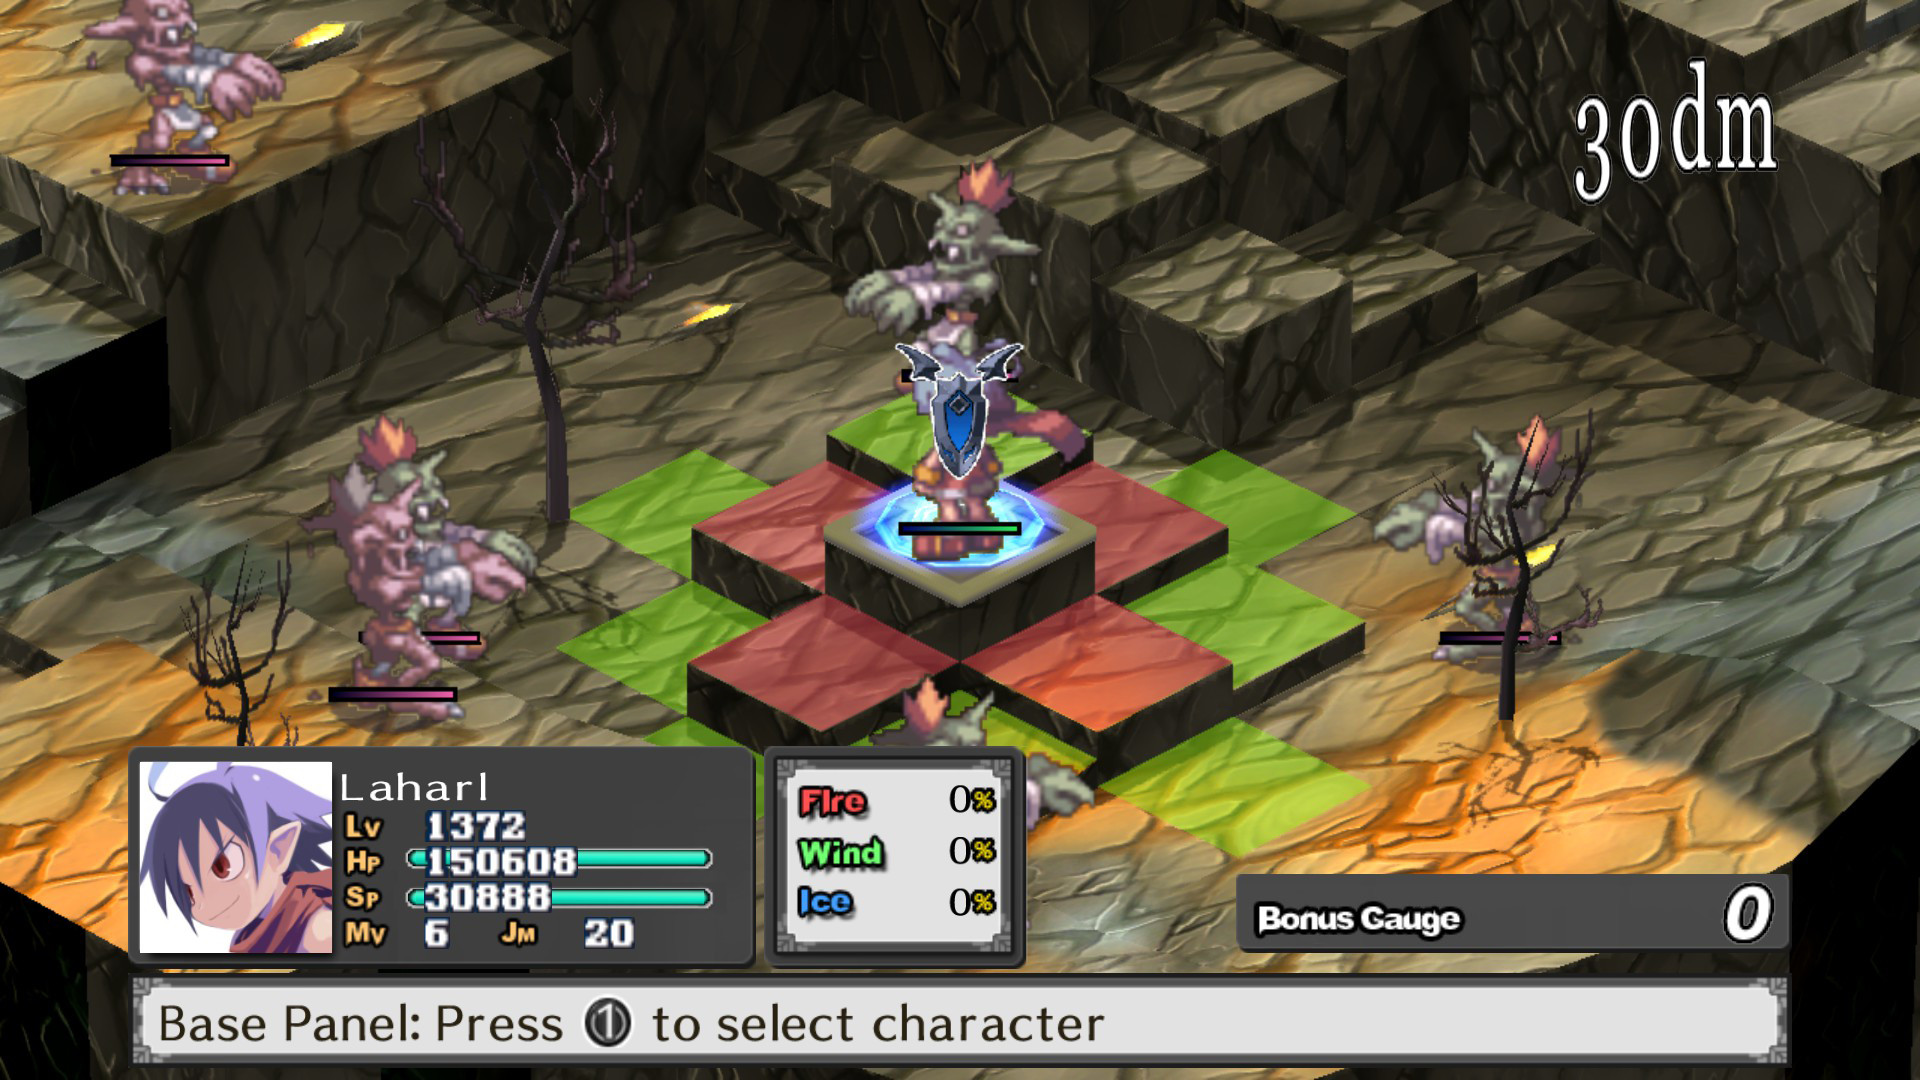
\includegraphics[width=\linewidth]{images/disgaea_exemple.png}
\centering
\caption{Aperçu de l'ecran de Jeu du jeu Disgaea}
\label{fig:img1}
\end{figure}



\section{Règles du Jeu}


\subsection{But du Jeu}
Les joueurs ont chacun un nombre défini de troupes positionné sur la carte.
Le But du jeu est d'éliminer l'ensemble des troupes ennemies (condition de victoire).
Ou d'avoir toutes ses troupes éliminées (condition de défaite).
\\
Une unité est considérée comme détruire lorsque ses points de vie tombent à 0.

\subsection{Tour de Jeu}
Le jeu se découpe en une sucession de tours. Les joueurs jouent les uns à la suite des autres.

Dans un tour, le joueur peut: \\

\begin{itemize}
  \item Déplacer ses unités sur la carte sur un nombre limité de cases.
  \item Attaquer avec ses unités des unités adverses adjacentes ou à distance en fonction du type d'attaque utilisable par l'unité. 
  \item Appliquer une posture de défense sur ses unités pour augmenter la défense si attaquée. 
  \item Utiliser des objets sur ses unités pour la soigner etc...

\end{itemize}

\subsection{Terrain de Jeu}

Le terrain est décomposé en tuiles. Une unité reçoit des bonus ou des malus en fonction de la tuile sur laquelle elle se trouve. Une unité placée sur une tuile de forêt par exemple recevra un bonus d'esquive si attaquée.\\

Les tuiles peuvent avoir des hauteurs différentes. Une unité placée sur une tuile en hauteur aura une meilleure portée pour des attaques à distance, mais y accèder coûte plus de points de déplacement.

\section{Ressources}

\begin{figure}[H]
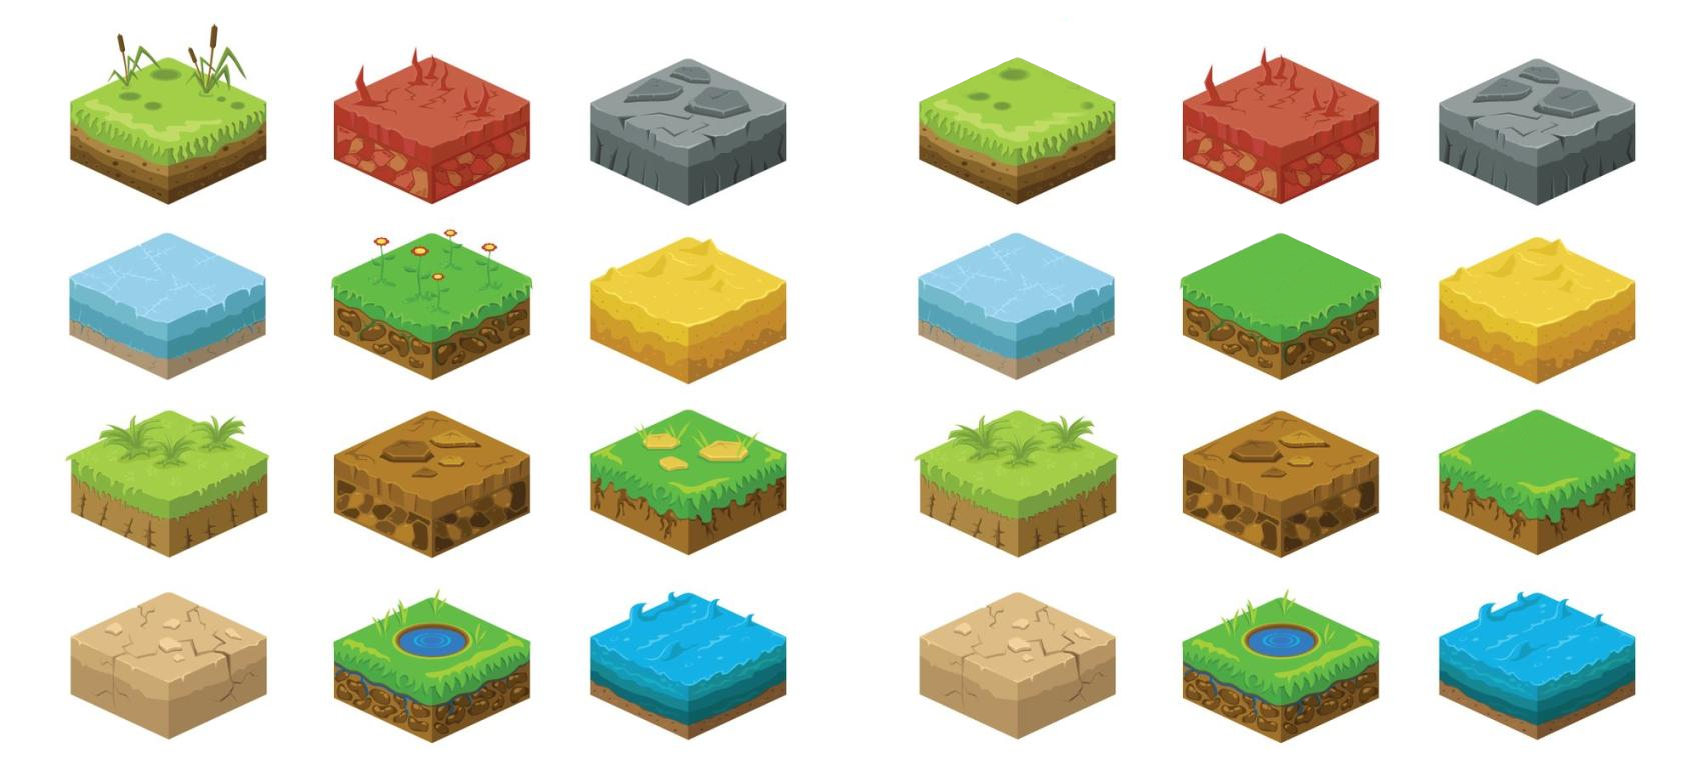
\includegraphics[width=\linewidth]{images/maptiles.png}
\centering
\caption{Tiles pour la carte en perspective isométrique}
\label{fig:img2}
\end{figure}

\begin{figure}[H]
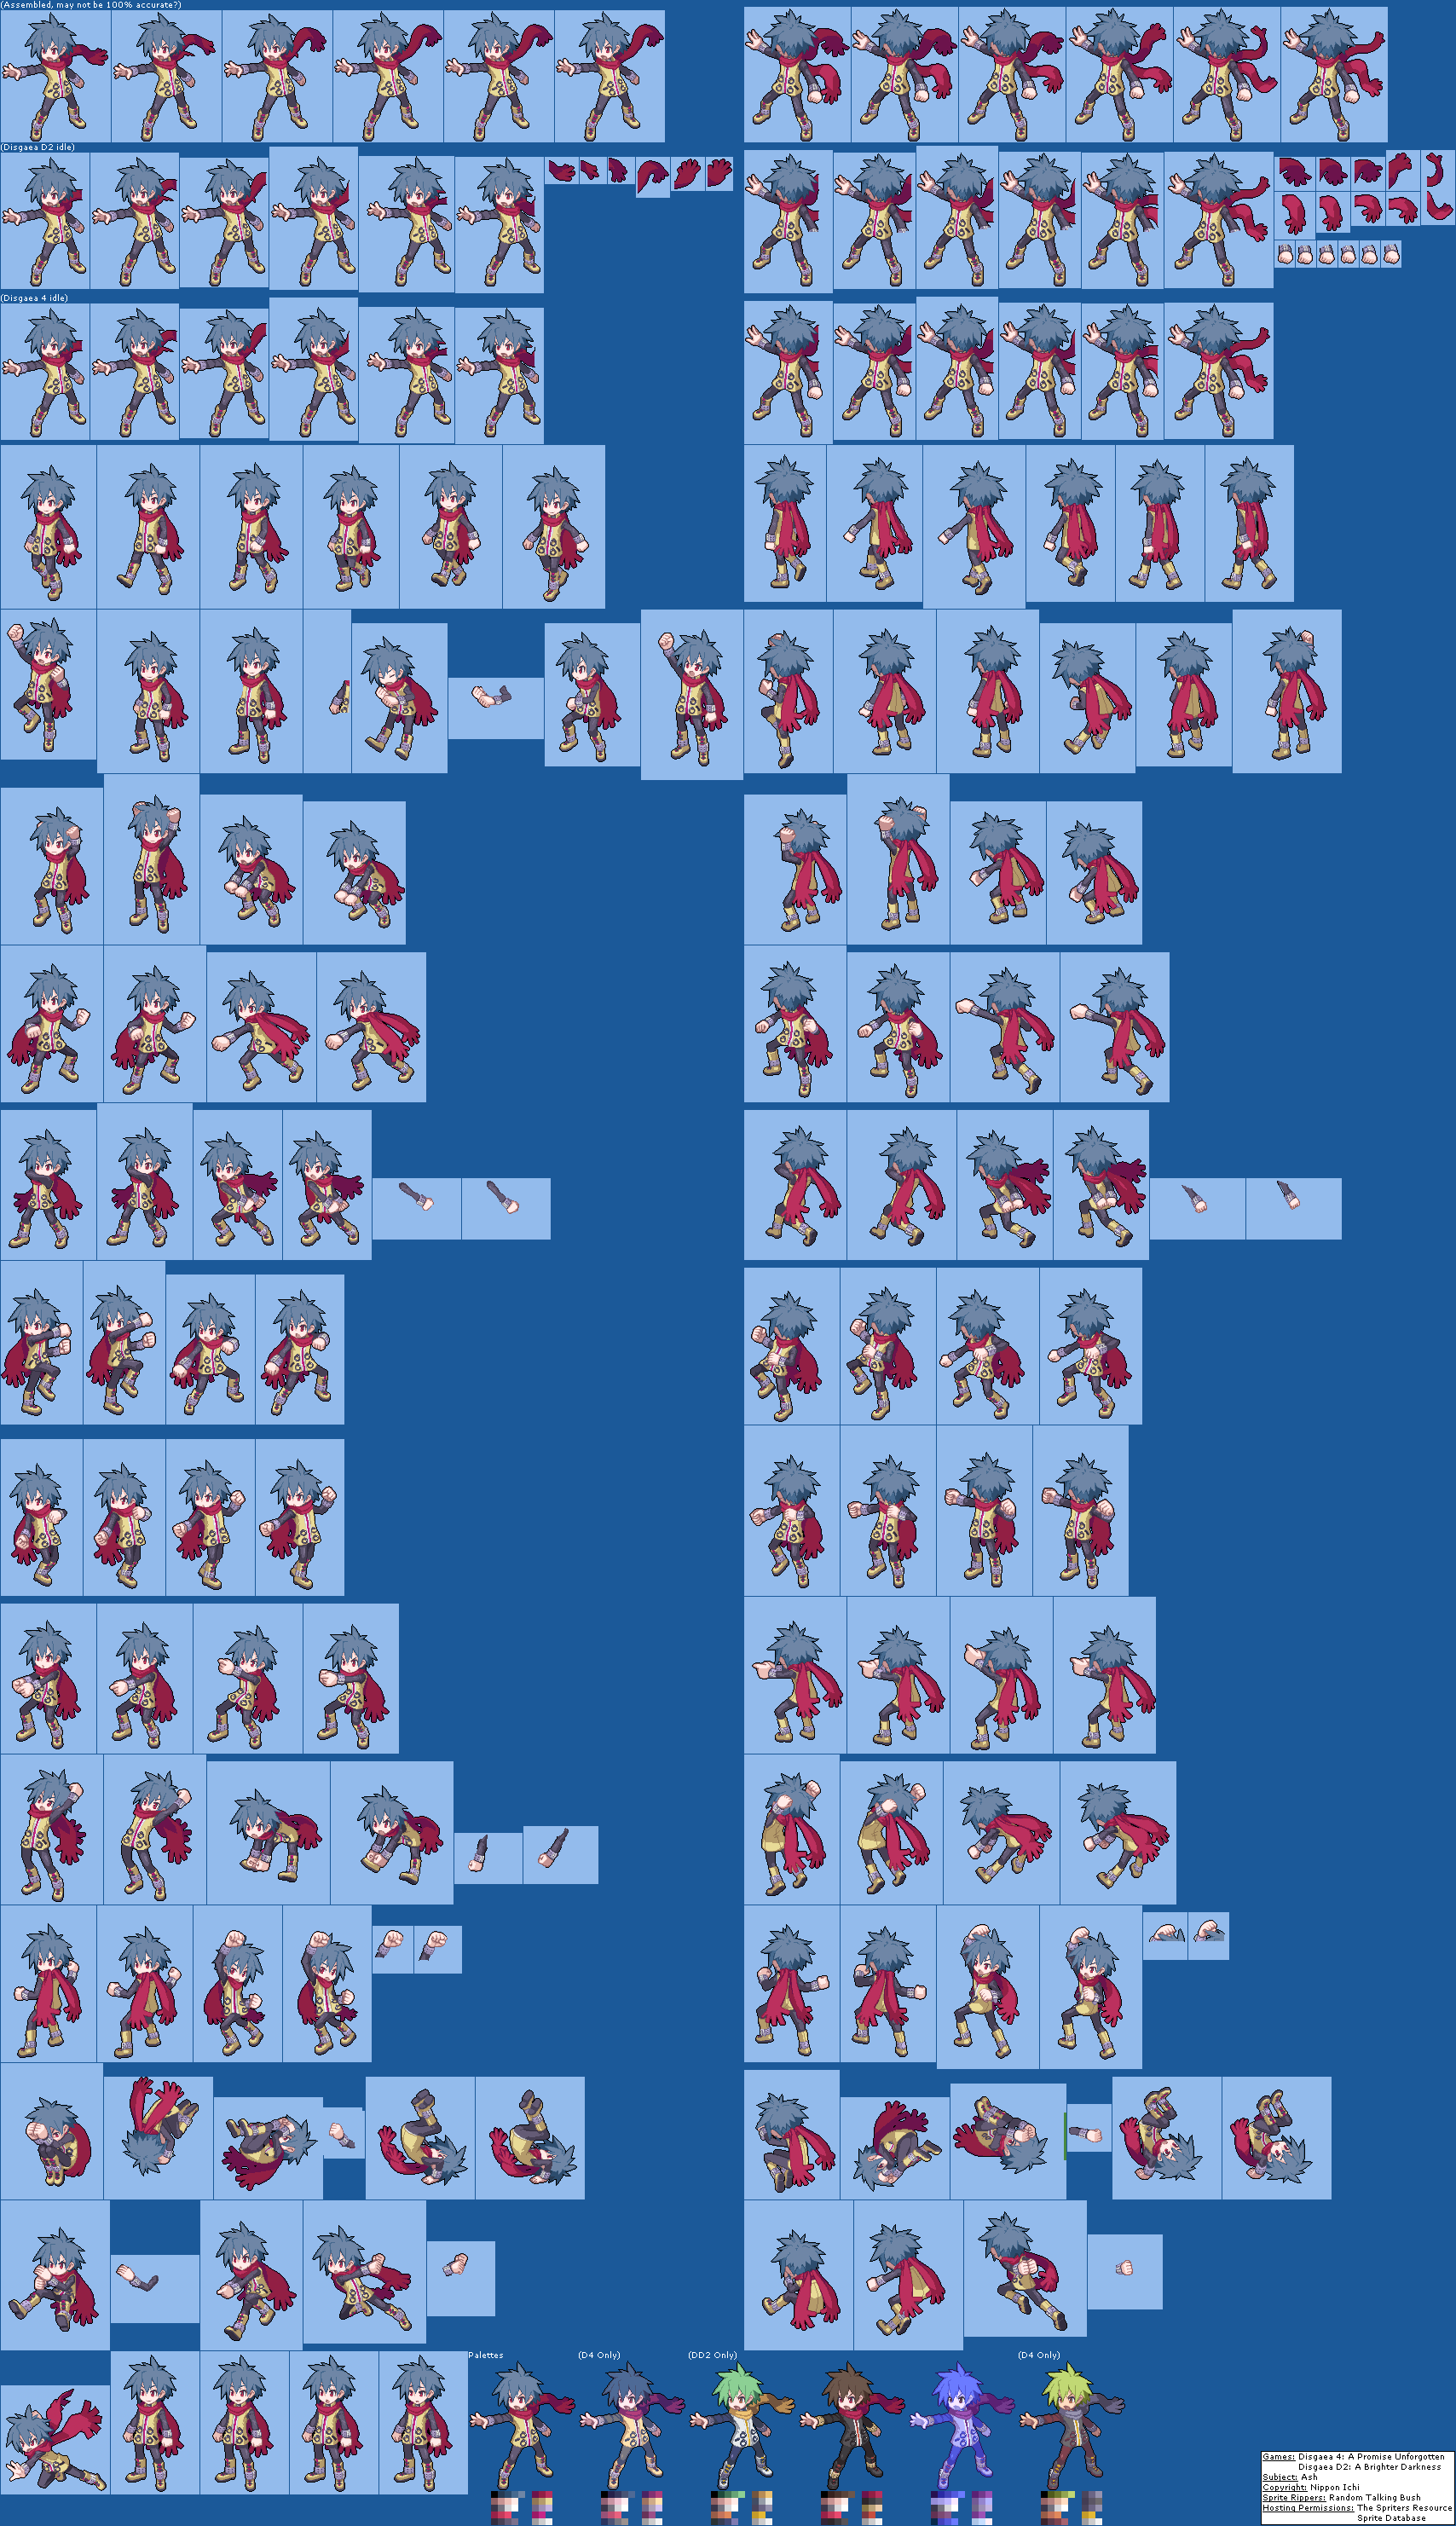
\includegraphics[scale=0.15]{images/char1.png}
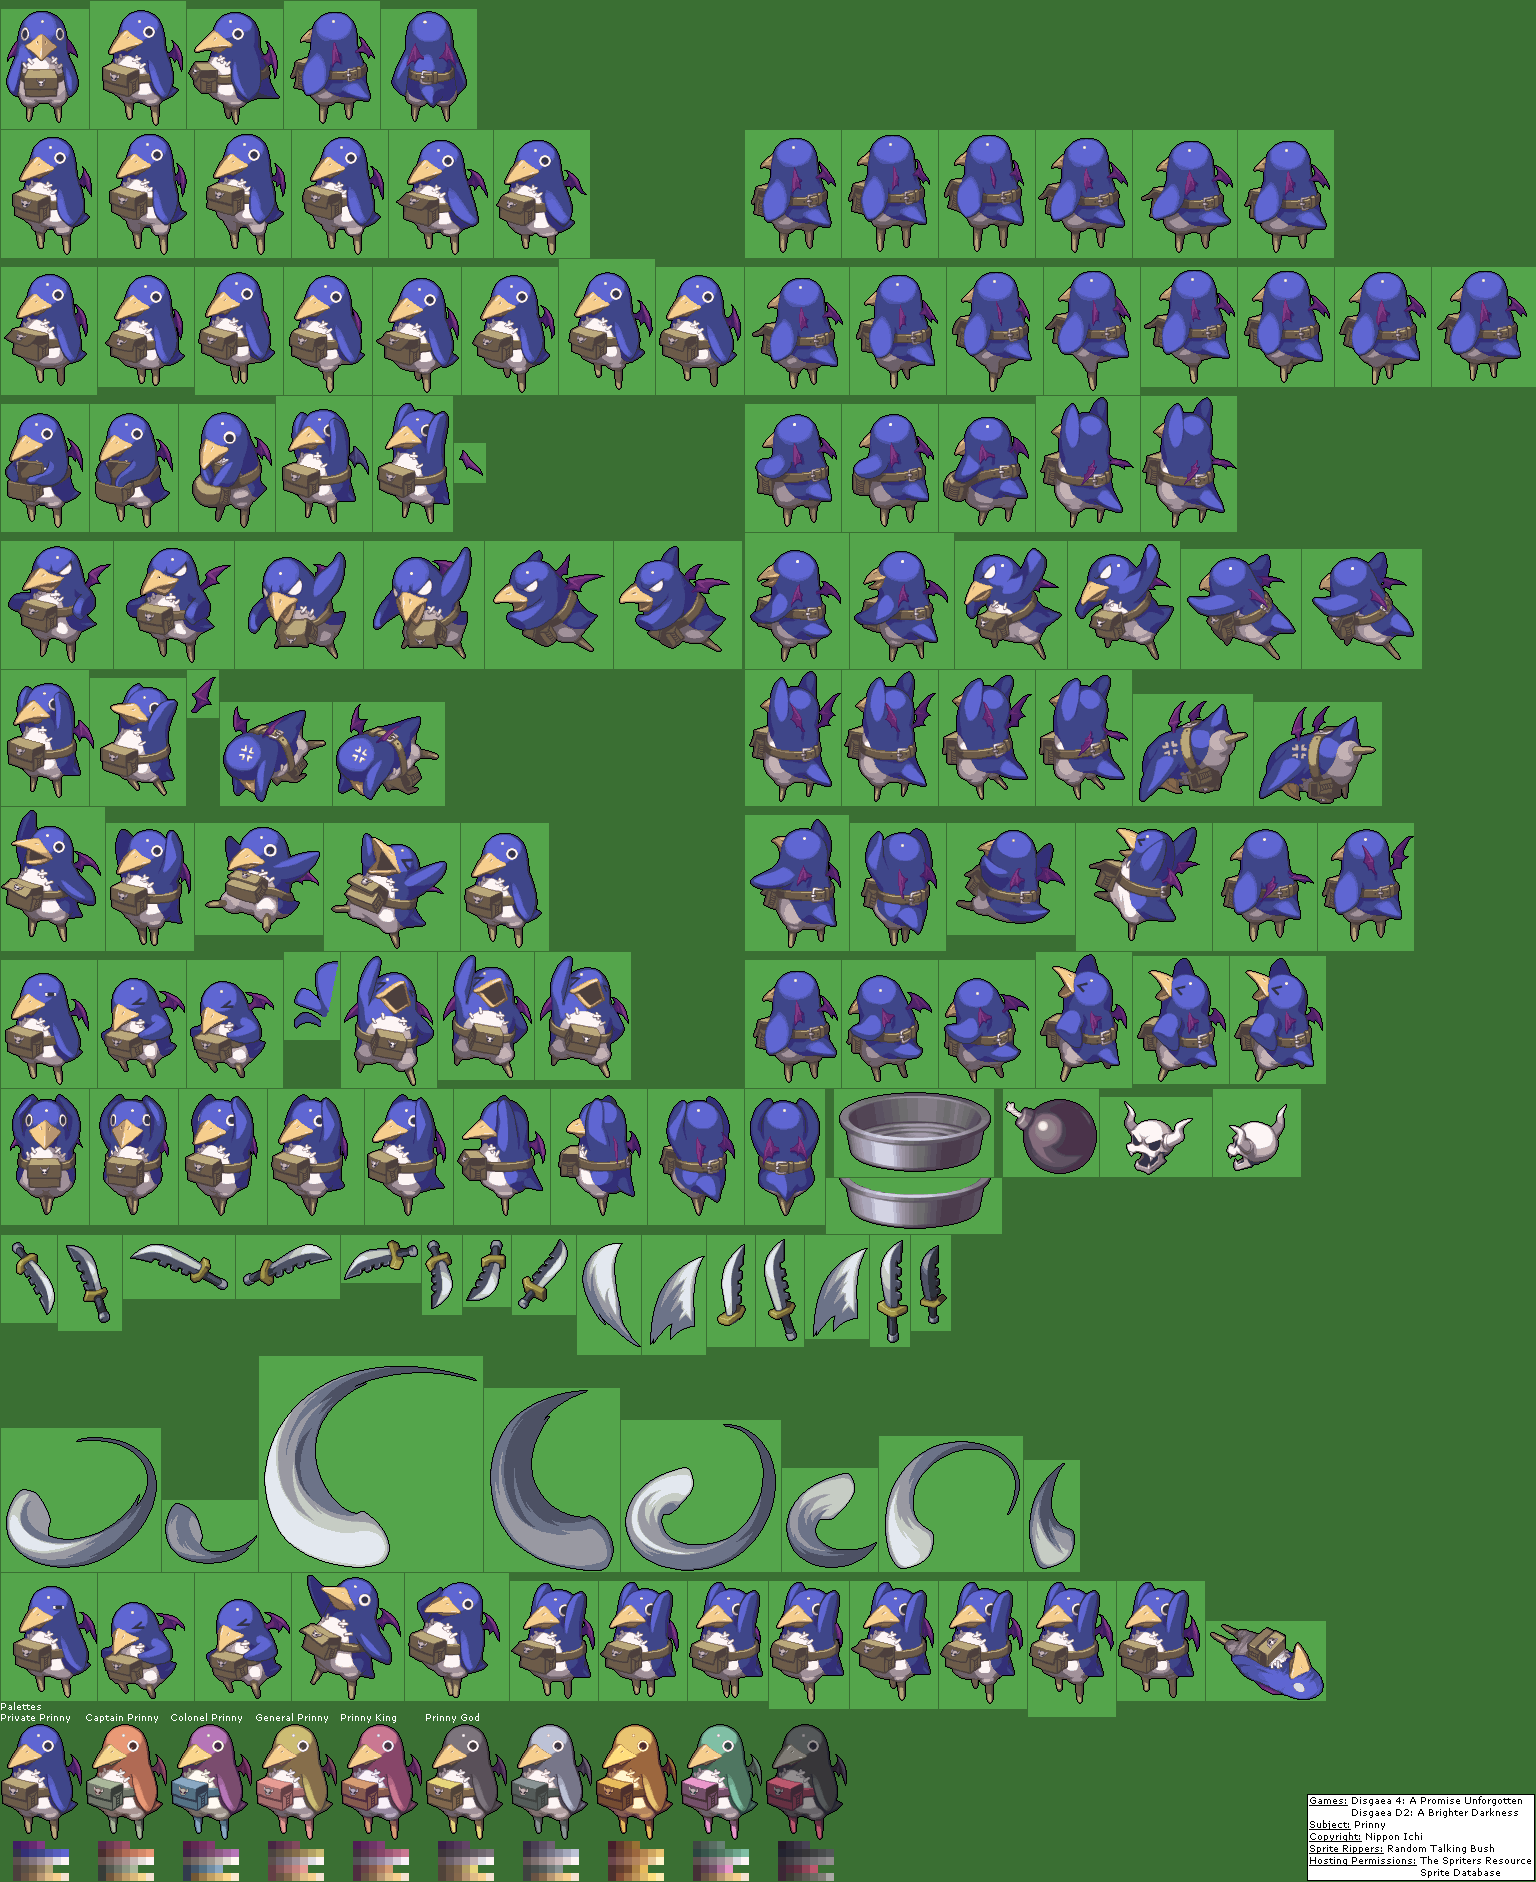
\includegraphics[scale=0.15]{images/enn1.png}
\centering
\caption{Spritesheets personnages}
\label{fig:img3}
\end{figure}

\chapter{Description et Conception des états}


\section{Description des états}

Dans un état du jeu, on retrouve des éléments fixes: les tiles (tuiles isometriques) qui composent la carte et des éléments mobiles: les personnages. Tous les éléments ont un nom et une position.

\subsection{Etat éléments fixes}

La carte du jeu est une table à 2 dimensions composée de tuiles.

Les tuiles sont générées de manière aléatoires. 
On retrouve dans les propriétés des tuiles : 
\\

\begin{itemize}
    \item \textbf{le type de tuile:} Il est critère de praticabilité pour un personnage et aussi pour l'affichage du sprite correspondant côté gestion rendu.
       \begin{itemize}
         \item[•]  Dirt
         \item[•]  Grass
         \item[•]  Water
         \item[•]  Sand
         \item[•]  Pound
         \item[•]  Rock
         \\
       \end{itemize}
    Les effets des types seront déterminés côté engine en fonction du type de tuile.
    \\
    \item \textbf{la hauteur:} Elle determine la hauteur de la tuile, modifieur impactant la distance de déplacement dans les actions et la portée d'une attaque qui seront gérés dans la partie engine. La hauteur est un entier compris entre 1 et 3.
\end{itemize}

\subsection{Etat éléments mobiles}

Les personnages appatiennent à des équipes. Chaque équipe est gérée par un joueur.  
Un personnage possède:
\\
\begin{itemize}
\item Une race générée aléatoirement parmi la liste suivante:
    \begin{itemize}
         \item[•]  Monster
         \item[•]  Beastman
         \item[•]  Demon
         \item[•]  Human
         \\
     \end{itemize}

\item Un job généré aléatoirement parmi la liste suivante:
    \begin{itemize}
         \item[•]  Pugilist
         \item[•]  Swordsman
         \item[•]  Archer
         \item[•]  Magician
         \\
     \end{itemize}
\item Un niveau calculé en fonction de l'expérience amassée.
\\ \\
Les caractéristiques (PV max, PM max, dégâts physiques, dégâts magiques, score d'évasion, score de défense, liste des compétences) sont déterminés en fonctions des 3 attributs précédents (race,job et niveau).
\\
\end{itemize}

Un curseur permet aux joueurs de navigueur sur les tuiles et lire les propriétés 
(du terrain et d'un personnage si présent) et sélectionner un personnage (si présent) en vue d'effectuer une action.


\subsection{Etat général}
En plus des éléments statiques et mobiles nous avons :
\begin{itemize}
         \item \textbf{nombre de tour:} Le nombre de tours qui ont été joués.
         \\
         \item \textbf{terminé:} Un booléen qui indique si le combat est terminé.
\end{itemize}

\section{Conception Logiciel}
Le diagramme des classes UML C++ pour les états est visible en Figure X. Nous pouvons mettre en évidence plusieurs groupes de classes qui sont les suivants :
\\
\begin{itemize}
    \item Groupe Character (bleu foncé): Toutes les charactéristiques des personnages, qu'ils soient ceux du joueur ou non, ainsi que les fonctions pour y accéder. Il présente une hiérarchie des classes filles permettant de visualiser les différentes catégories associées aux personnages et les types de chacun de ses élements.
    \\
    \item Groupe Team (bleu clair): Principalement composé de la classe Team, cette dernière englobe les ressources d'un joueur à savoir ses personnages et ses objets.
    \\
    \item Groupe Entity (jaune): La gestion du curseur et de l'entité pointée par ce dernier pour afficher les propriétés de la tuile à l'écran et selectionner le personnage qui réalise une action. 
    \\
    \item Groupe Observante (orange): Il sera implémenté en parallèle avec le render, pour pouvoir faire les tests.
    \\
    \item Groupe Turn (vert): Il représente l'état général durant un tour.
    \\
    \item Groupe Tile (gris): Ce groupe permet la construction d'une Tile aléatoire à l'aide de TileFactory. La carte sera formée à partir de ces Tiles. 
\end{itemize}

\section{Tests Unitaires}

Des tests unitaires ont été réalisés pour vérifier les fonctions des différentes classes. On réalise un fichier de test par classe.
Le code est couvert aux alentours de 88\% par les tests unitaires.

\newpage

\begin{figure}[H]
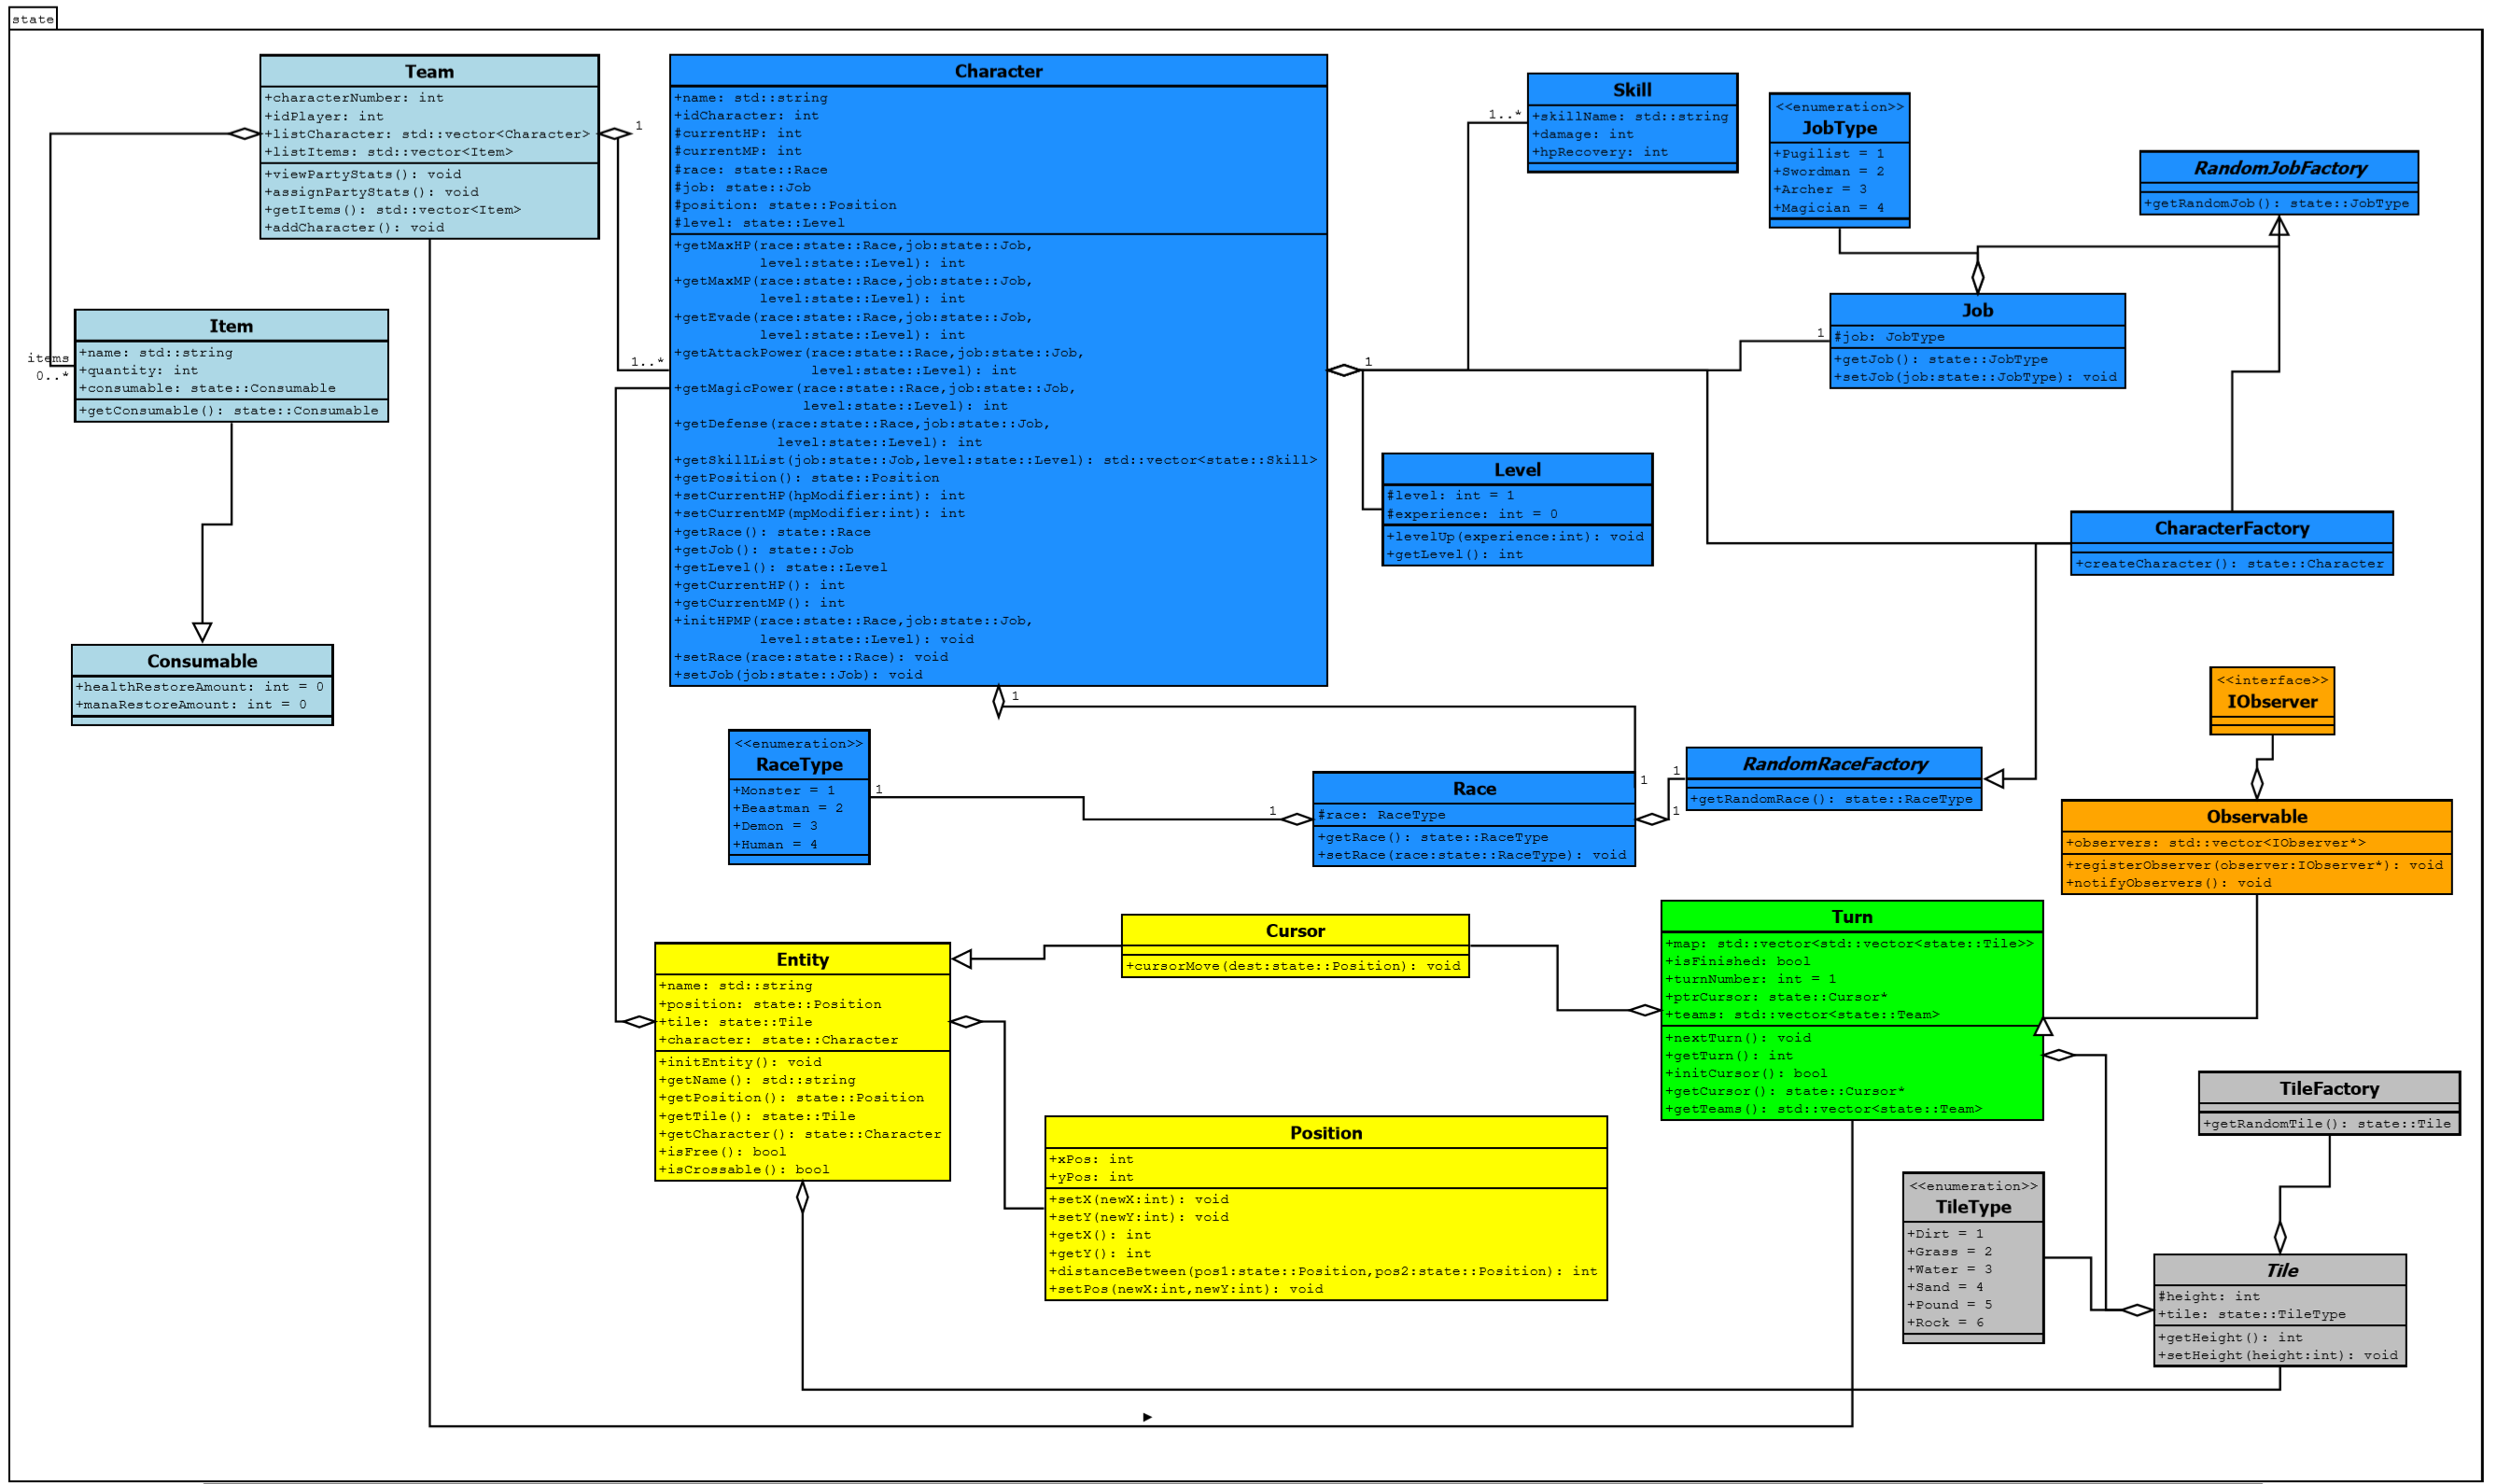
\includegraphics[width=\linewidth]{images/states.png}
\centering
\caption{Aperçu de state.dia}
\label{fig:img3}
\end{figure}
\newpage
\chapter{Description et Conception du rendu}


\section{Description de la stratégie de rendu d’un état}

Pour le rendu d'un état nous avons décidé de réaliser une vue isométrique 
à l'aide de la librairie SFML de notre carte générée
aléatoirement. Il est possible de faire entrer en rotation la vue avec les
touches R et T, et déplacer la vue avec les touches directionnelles. 
\\
\\Nous découpons la scène à rendre en couches (ou « layers ») : une couche 
pour chaque hauteur de tuile (1 à 3) et une couche par personnages.
Chacunes des couches de tuile est divisé en deux : les murs et le
plafonds. Le plafond d'une couche à la priorité sur les murs de
cette même couche et une couche supérieure à priorité sur une
couche inférieure.
\\
\\Chaque couche contiendra des informations qui seront utilisées
par la libraire Sfml : un unique tileset contenant les tuiles 
(ou « tiles »), et une unique matrice avec 
la position des éléments et les coordonnées dans la texture.
\\
\\En ce qui concerne les aspects de synchronisation, nous avons 
une horloge à 60Hz qui permet l'actualisation du rendu. 
De plus, nous avons aussi les animations des personnages 
fixes qui arrivent toutes les 60ms (soit environ 17Hz).

\section{Conception Logiciel}

Le diagramme des classes UML C++ pour le rendu est visible en Figure 3.3.

On divise le Rendu en 3 classes:

\begin{itemize}
    \item \textbf{La classe TileSet:} Elle est constitué d'un constructeur où l'on précise le type (Maptile, CharaSpritesheet) pour créer un objet TileSet avec:
    \begin{itemize}
         \item[•]  le chemin vers le tileset (imagePath)
         \item[•]  la taille horizontale d'une tuile (sizeX)
         \item[•]  la taille verticale d'une tuile (sizeY)
         \item[•]  la marge, espace entre les tuiles (margin)
         \\
    \end{itemize}     
    \item \textbf{La classe DrawObject:} Elle regroupe les fonctions de rendu des objets (plafonds,murs et personnages)
    et une fonction virtuelle draw redéfinie de la librairie sfml.
    \\
    Elle possède 2 attributs utiles au rendu: un objet texture de la librairie sfml et un tableau de vertex.
    \\
    Pour réaliser le rendu isométrique de la carte, on écrit les coordonnées X et Y iso dans le repère Cartésien. 
    \\Et on définit nos vertex comme suivant:
    
\begin{figure}[H]
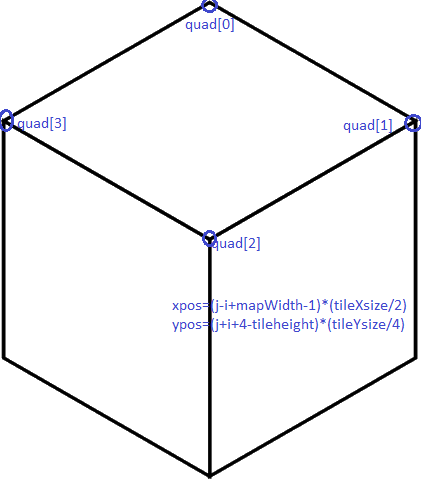
\includegraphics[]{images/carre_iso.png}
\centering
\caption{Schema calcul position isometrique}
\label{fig:img3}
\end{figure}

                quad[0].position = sf::Vector2f(xpos + tileXsize/2     , ypos + tileYsize/2    );
                \\quad[1].position = sf::Vector2f(xpos + tileXsize     , ypos + 3*(tileYsize/4)     );
                \\quad[2].position = sf::Vector2f(xpos + tileXsize/2   , ypos + tileYsize         );
                \\quad[3].position = sf::Vector2f(xpos                 , ypos + 3*(tileYsize/4)   );
\\
\\
    \item \textbf{La classe TurnDisplay:} La classe TurnDisplay est 
    constituée d'un constructeur qui génère un objet TurnDisplay pour un tour (turn) donné. 
    Il possède la réference à ce tour,
    une liste de tilesets et une liste de drawobjects vide.
    Sa fonction initRender appelle 
    les fonctions d'une instance de DrawObject 
    et les append à sa liste de drawobjects. 
    \\
    Pour les personnages, on fait un tableau à 2 dimensions pour
    stocker chaque sprites de l'animation des personnages.
\end{itemize}

\begin{figure}[H]
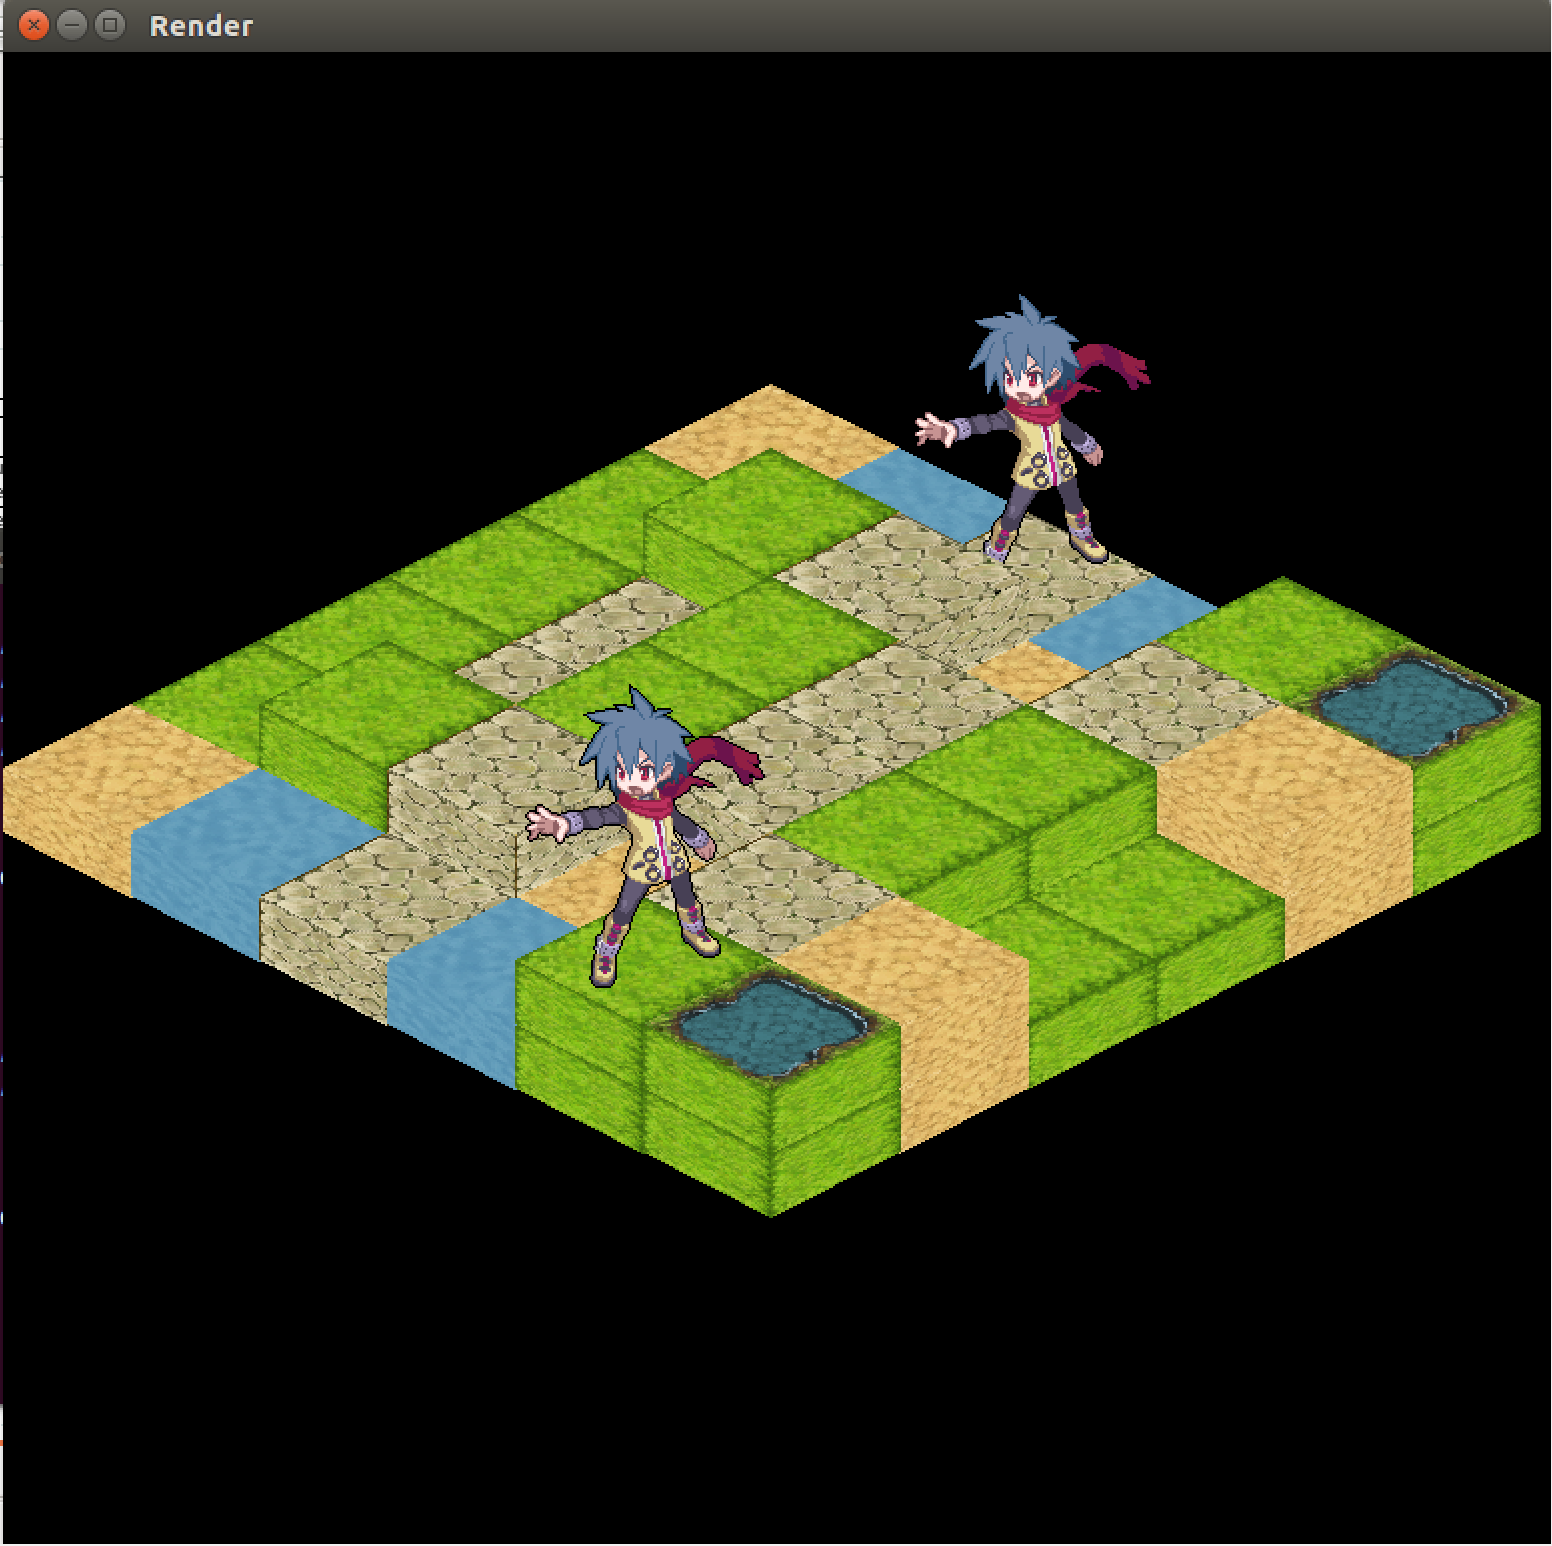
\includegraphics[width=\linewidth]{images/RenderPreview.png}
\centering
\caption{Aperçu du rendu d'un etat de jeu}
\label{fig:img4}
\end{figure}

\begin{figure}[H]
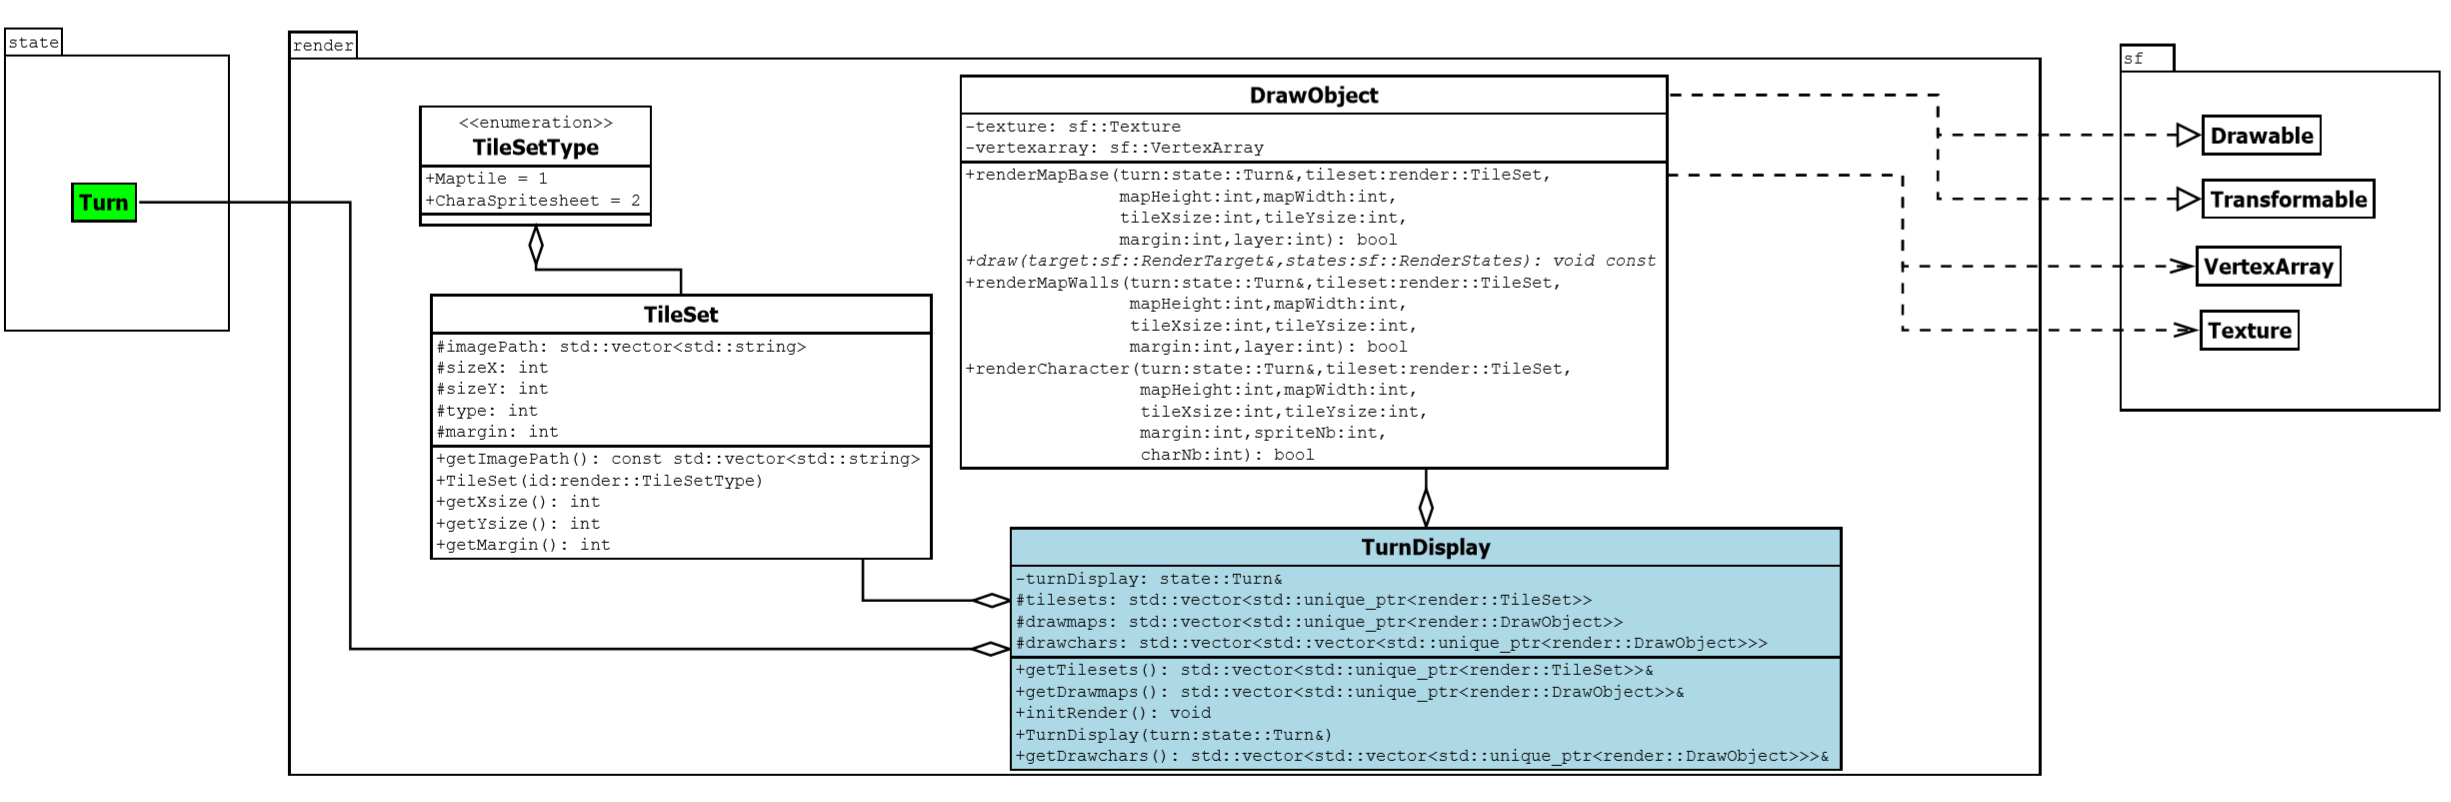
\includegraphics[width=\linewidth]{images/renderdia.png}
\centering
\caption{Aperçu de render.dia}
\label{fig:img5}
\end{figure}

\chapter{Règles de changement d’états et moteur de jeu}

\section{Règles de changement d’états}

Le tour de jeu d’un joueur est terminé lorsque tous ses personnages possèdent un statut USED ou DEFENDING.
\\Les actions sont réalisées en fin de tour dans l'ordre entré par le joueur actif. 
C’est alors le tour du joueur adverse.
\\Lorsqu’un personnage est attaqué par un ennemi, il perd des points de vies correspondant à 
l'attaque de l'attaquant moins sa défense.
Lorsqu’un personnage utilise un objet, il peut l'utiliser sur lui-même ou sur 
un autre personnage, pour gagner des points de vie par exemple.
\\Si un personnage perd tous ses points de vie, son statut évolue et prend la valeur DEAD.
Si tous les personnages d’un joueur meurent, la partie est terminée 
à la fin du tour et le joueur adverse gagne.
\\Chaque action effectuée modifie l’état des personnages concernés, 
autant celui la réalisant que les victimes. 
Le choix du personnage sélectionné et des actions effectuées est provoqué par des commandes.
Pour ce jalon une séquence de commande est réalisée dans le fichier "main.cpp".
\\Le scénario de test comporte 5 tours, on peut jouer un tour en appuyant sur la touche E.


\section{Conception logicielle}
Le diagramme des classes UML C++ pour le moteur est visible en Figure 4.1.
On divise le moteur de jeu en 3 groupes de classes.
\begin{itemize}
    \item \textbf{Le agroupe de la classe Engine:} C’est le coeur du moteur du jeu. 
    Cette classe permet de stocker les commandes dans un vecteur de Command (avec l'opération "addCommand"). 
    Ce mode de stockage permet d’introduire une notion d'ordre: on réalisé les commandes dans 
    l'ordre où le joueur les à rentrées. Lorsque turnCheckOut est appelé les commandes sont exécutées, 
    si tout les personnages ont des actions ou s'ils passent leur tour, puis on change de joueur actif.
    \\
    \item \textbf{Le groupe de la classe Command:} C'est la classe maîtresse des actions. 
    Elle définie les méthodes de manière abstraite afin quelles soient utilisables et 
    modifiables par toutes les actions grâce au polimorphisme.
    \\
    \item \textbf{Le groupe des classes Attack, Defend, Move, EndTurn, UseObject et UseSkill:} 
    Les classes Attack, Defend, Move, EndTurn, UseObject et UseSkill, héritant de la classe
    Command, possèdent chacune une méthode "validate" qui permet de savoir si le personnage et 
    capable de réalisé la commande et une méthode "action" qui fait exécuté au personnage 
    l’action correspondante à la commande. Chacun possède aussi un constructeur permettant de 
    savoir quel personnage réalise l'action, quel(s) personnage subit l'action et les spécificités 
    liées à chacune des actions.
\end{itemize}



\begin{figure}[H]
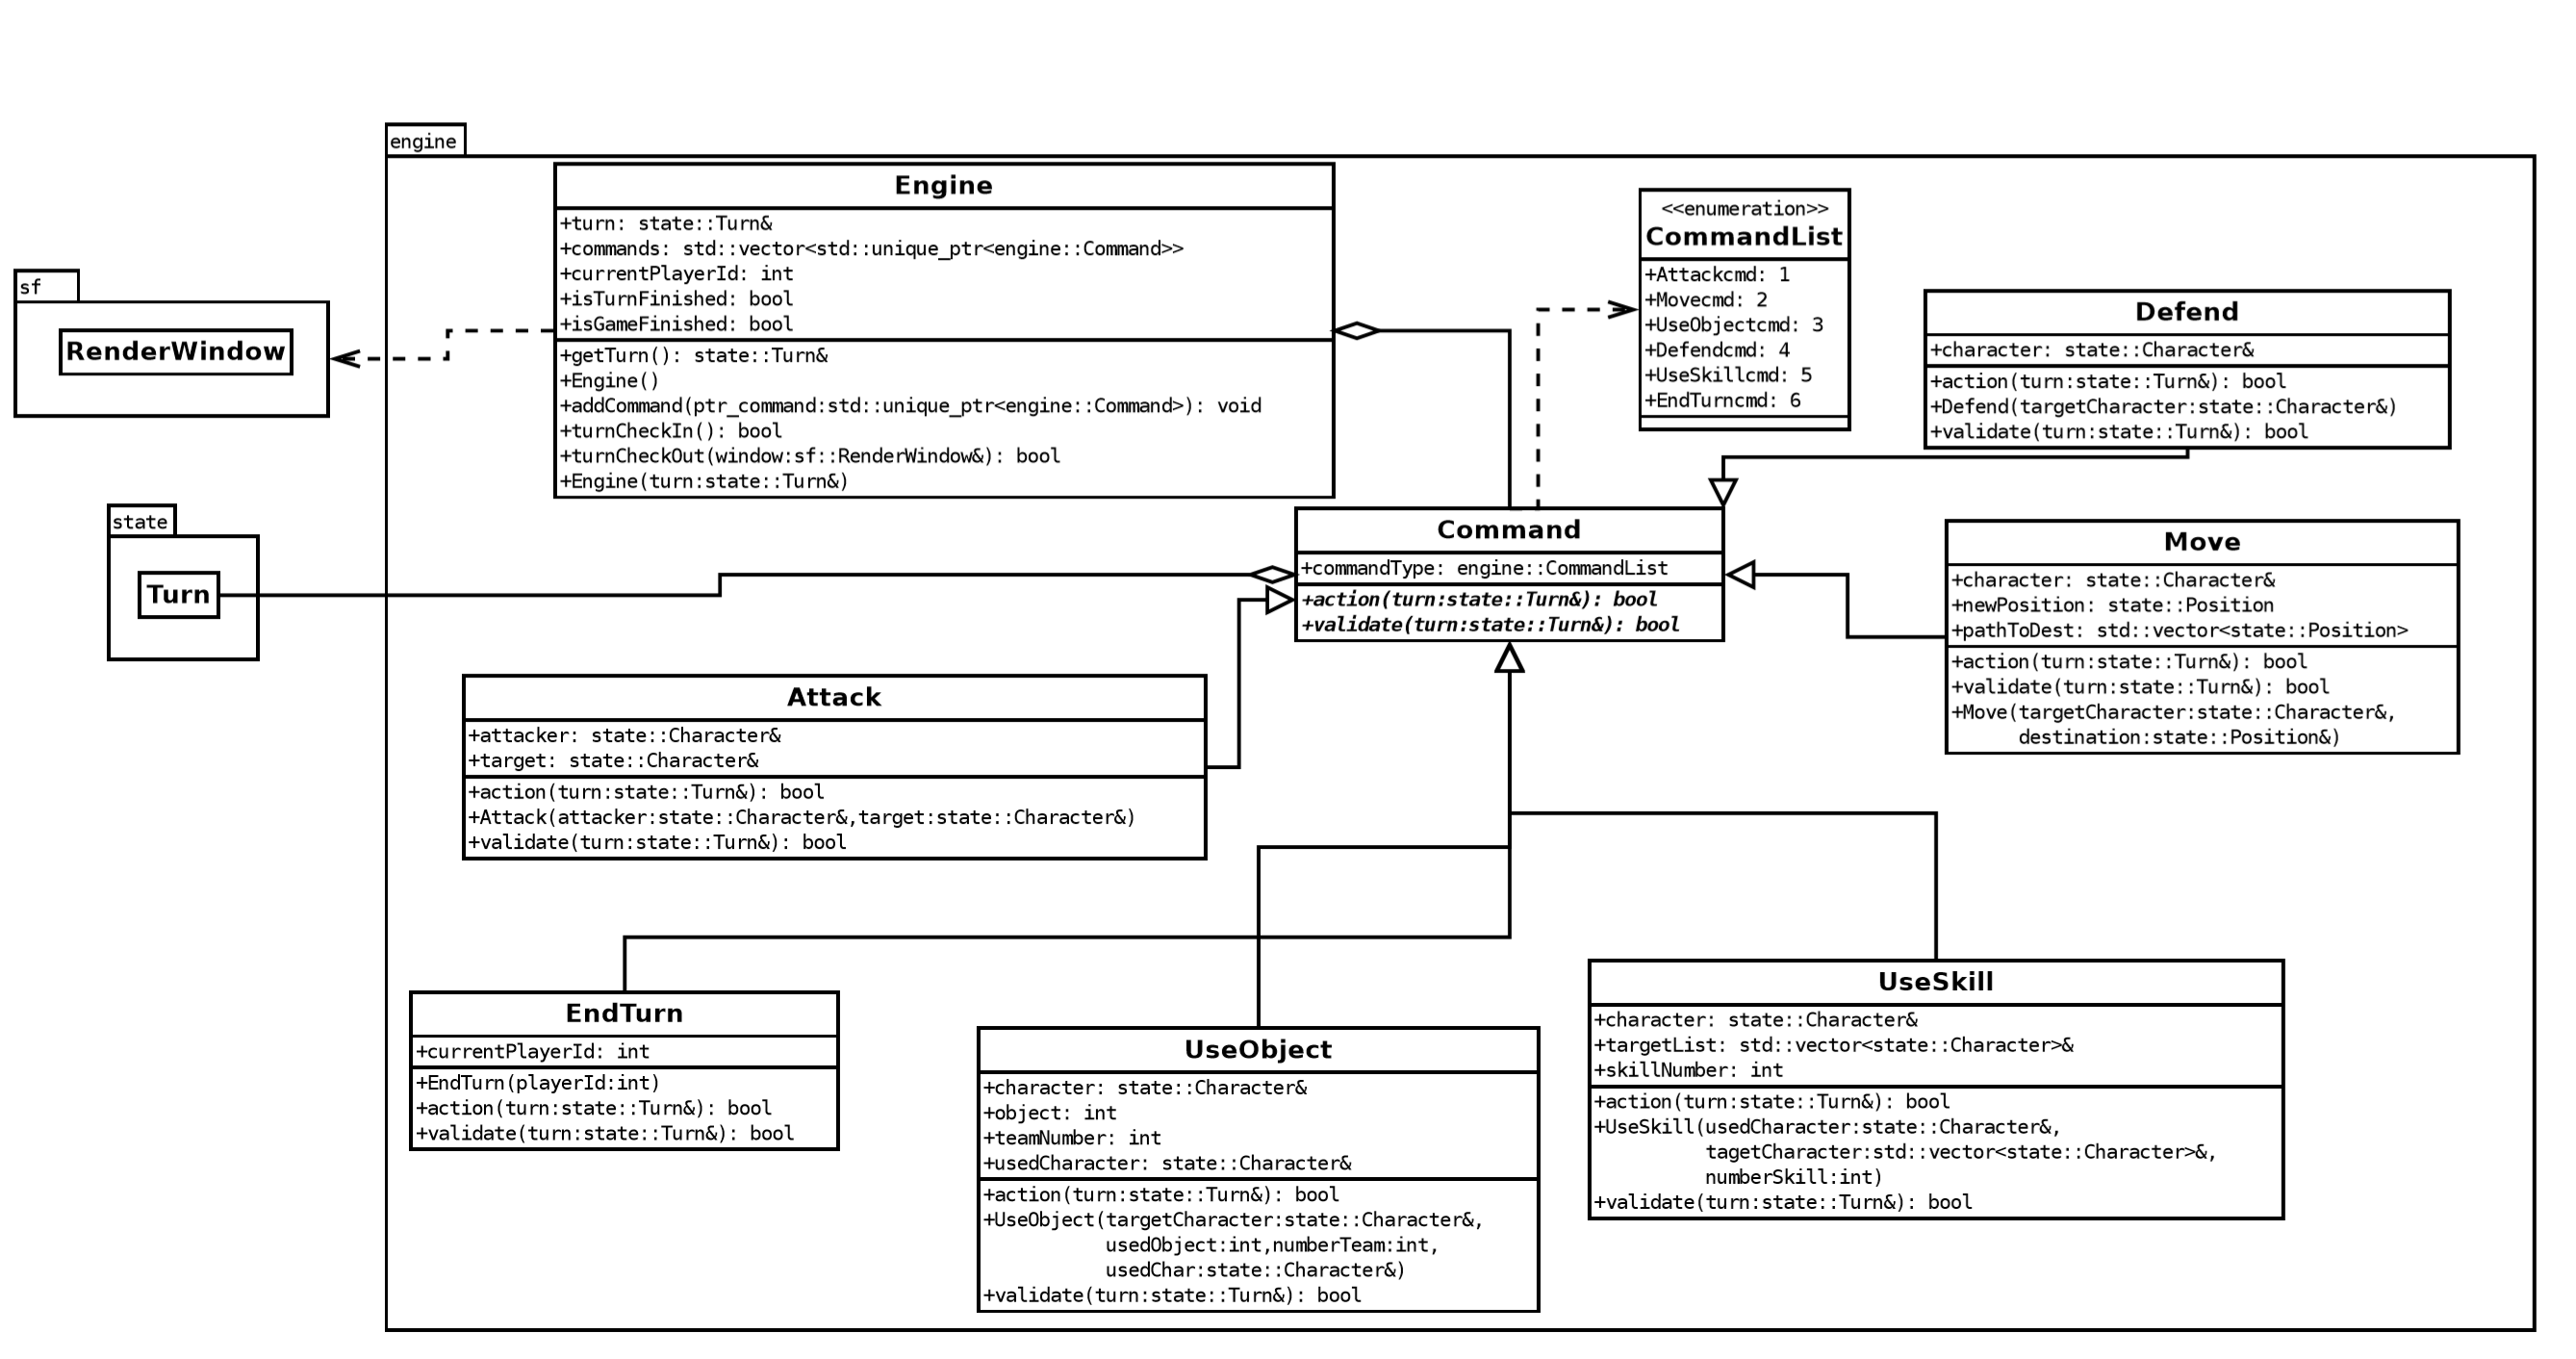
\includegraphics[width=\linewidth]{images/engine_dia.png}
\centering
\caption{Aperçu de engine.dia}
\label{fig:img3}
\end{figure}

\chapter{Intelligence Artificielle}

\section{Stratégies}

\subsection{Intelligence Aléatoire}

L’ IA contrôle une liste de personnages appartenant au joueur actuel,
elle va les sélectionner les uns après les autres lors de son tour 
de jeu.
Une fois un personnage sélectionné, un entier correspondant à une 
action précise est choisi au hasard parmi 6 : 1 (attaquer), 2 (se 
déplacer), 3 (utiliser un objet), 4 (défendre), 5 (utiliser une 
compétence) et 6 (passer son tour).
\\\\
Lorsqu'une action est séléctionnée on teste sa faisabilité, sinon un 
nouveau nombre est séléctionné jusqu'à ce que l'action soit valide. 
\\\\
Si l'action est possible alors elle est ajoutée à la liste des 
commandes et l'IA passe au personnage suivant.
\\\\
Si "attaquer" est choisie, une cible va être déterminée aléatoirement
parmi tout les autres personnages, y compris ceux de son équipe. Si 
la cible de l'attaque est trop éloignée alors l’attaque n’aura pas 
lieu, si la distance entre les deux personnages est suffisante alors 
l'attaque est ajoutée à la liste des commandes.
\\\\
Si "se déplacer" est choisie, le personnage sélectionné tente de se 
mouvoir sur une case aléatoire, si cela est réalisable alors le 
déplacement est ajouté à la liste des commandes.
\\\\
Si "utiliser un objet" est choisie, alors le personnage va utiliser 
un objet aléatoire de la liste des objets appartenant à son équipe, 
puis il applique l'effet sur une cible aléatoire, si l'objet est en 
quantité suffisante alors l'action est ajoutée à la liste des 
commandes.
\\\\
Si "défendre" est choisie, le personnage sélectionné se met en 
position défensive, dans le cas présent puisque l'on cherche les 
actions des personnages dans l'ordre, cette action ne peut échouer 
puisque le personnage n'a pas d'autres actions dans la liste, 
l'action "défendre" est donc ajoutée à la liste.
\\\\
Si "utiliser une compétence" est choisie, alors le personnage va 
utiliser une compétence aléatoire de la liste des compétance qu'il 
peut utiliser, puis il applique l'effet sur une cible aléatoire, si 
la distance entre lui et sa cible est inférieure à la distance 
maximum de la compétence alors la compétence est ajoutée à la liste 
des commandes.
\\\\
Si "passer son tour" est choisie, l'IA termine son tour d’action.
Lorsque passer son tour ou lorsque tout les personnages de l'équipe 
du joueur actuel ont une action, alors cela fini ainsi la liste des 
commandes, les commandes sont exécutées dans l'ordre de la liste. 
Puis c'est au tour de l'adversaire.
\\

\subsection{Intelligence Heuristique}

L'IA heuristique fonctionne sur un système de point calculé pour 
chaque action possible.
L'IA va lister les actions possibles par personnages de son équipe et 
calculer un score pour chacune de ces actions.
Le score est calculé en fonction de la pertinence des actions.
\\\\
Concrètement, un personnage peut se déplacer puis effectuer une 
action ou seulement effectuer une action.
Il privilégiera des déplacements où les personnages adverses ne 
peuvent pas l'atteindre après déplacement ou bien s'il peut attaquer 
un unique ennemi avec un minimum d'attaque subit le tour suivant. 
C'est-à-dire en termes de point, plus il y a d'ennemis qui pourront 
l'attaquer au tour suivant plus il va perdre de point pour cette 
action, s'il y a un unique ennemi qu'il peut attaquer après son 
action de déplacement il va gagner des points. De plus il gagne des 
points suplémentaires s'il est hors de porté d'attaque et de 
déplacement puis attaque.
\\\\
Une attaque est privilégiée si l'ennemi est tué en conséquence de
l'action. Elle est priviligié si le personnage ne peut subir que peu 
d'attaques au prochain tour, sinon l'IA privilégie la défense qui réduit
grandement les dégats subits au prochain tour adverse.
En termes de point, une attaque rapporte plus de point qu'une action 
classique puisque le but du jeu est de tué les personnages adverses. 
Si une attaque tue un adversaire alors l'action rapporte encore plus 
de points.
\\\\
Un objet de soin n'est utilisé que lorsque celui-ci est nécessaire 
(vie<20\% ou mana<20\%) afin qu'il ne soit pas utilisé sur des cibles 
qui n'ont pas perdu des points de vie ou des points de mana comme 
pourrait le faire l'IA aléatoire.
En termes de point l'action perds des points si le personnage à son 
maximum de vie ou de mana, il gagne plus de point si les points de 
vie ou de mana sont sous le seuil critique (20\%).
\\\\
En terme de point une action défensive gagne de plus en plus de point plus il y a de personnages de l'adversaire qui pourront l'attaquer au prochain tour.
\\
\subsection{Intelligence Profonde}

L'IA profonde va lister les actions possibles par personnages 
de son équipe et calculer un score pour chacune de ces actions, comme le
fait l'IA heuristique. 
\\\\
On finit dans un premier temps le tour en cours en complétant la séquence
actuellement obtenue de l'IA profonde, par celle que l'on obtiendrait de
l'IA Heuristique.
\\\\
Le score est calculé après 2 tours de chaque équipe en considérant que
ces tours sont exécutés par l'intelligence heuristique, c'est-à-dire que
les tours sont réalisés dans l'optique d'obtenir les meilleures actions
possibles pour le tour en prédisant les coups de l'adversaire.
\\\\
On calcule le score en fonction des dégâts subis par l'équipe du joueur
et ceux subis par l'adversaire.
\\\\
Après le calcul du score on exécute les tours ainsi effectués dans le
sens inverse pour revenir au tour initial grâce au rollback implémenté.
La fonction revertTurn de Engine se charge de lancer les actions réciproques 
des actions exécutés durant un tour pour retourner au tour précédent et on 
décrémente le nombre de tours passés.
On s'évite ainsi de cloner l'objet turn.
\\\\
Après être revenu au tour actuel de jeu, on recharge la file d'actions retenues 
par l'IA profonde pour le tour en cours.
\\\\
Cette boucle est ainsi exécutée jusqu'à ce que plus aucun personnage ne 
puisse effectué d'actions. On exécute alors la liste des commandes
obtenues avec les meilleurs scores.

\section{Conception Logiciel}
Le diagramme des classes UML C++ pour l'intelligence artificielle est
visible en Figure 5.1.
On divise l'intelligence artificielle en 4 classes.
\\
\begin{itemize}

\item \textbf{AI :} C'est la classe principale, elle définie les 
méthodes qui serviront lors du polymorphisme lorsque les 
différentes IA seront appelées.
\\
\item \textbf{RandomAI :} C'est la classe représentant l'IA 
aléatoire, elle a une fonction pour determiner la liste des actions \\
des personnages controllé par l'IA (randomCommandList) et une 
fonction pour executer lancer l'IA (runAI).
\\
\item \textbf{HeuristicAI :} C'est la classe dédiée à l'IA heurisitique.
Elle comporte une fonction computeScore qui renvoie le score calculé
pour l'action donnée en entrée, une fonction heuristicCommandList pour
déterminer la liste des actions à partir des scores et une fonction
runAI pour lancer l'IA.
\\
\item \textbf{DeepAI :} C'est la classe de l'IA profonde. Elle comporte 
une fonction minMax qui renvoie le score en considérant le meilleur tour
de l'adversaire puis le meilleur tour du joueur (2 fois). 
Elle comporte aussi une fonction deepCommandList pour déterminer la liste des actions 
à partir des scores, une fonction runAI pour lancer l'IA.
Elle comporte également une fonction restoreCommandlist pour restorer 
la liste des actions en cours de construction après avoir fait deux tours 
de simulation et être retourné à l'état de tour actuel. La fonction updateQueue 
se charge de tenir à jour la file d'actions retenues par la deepIA.

\end{itemize}


\begin{figure}[H]
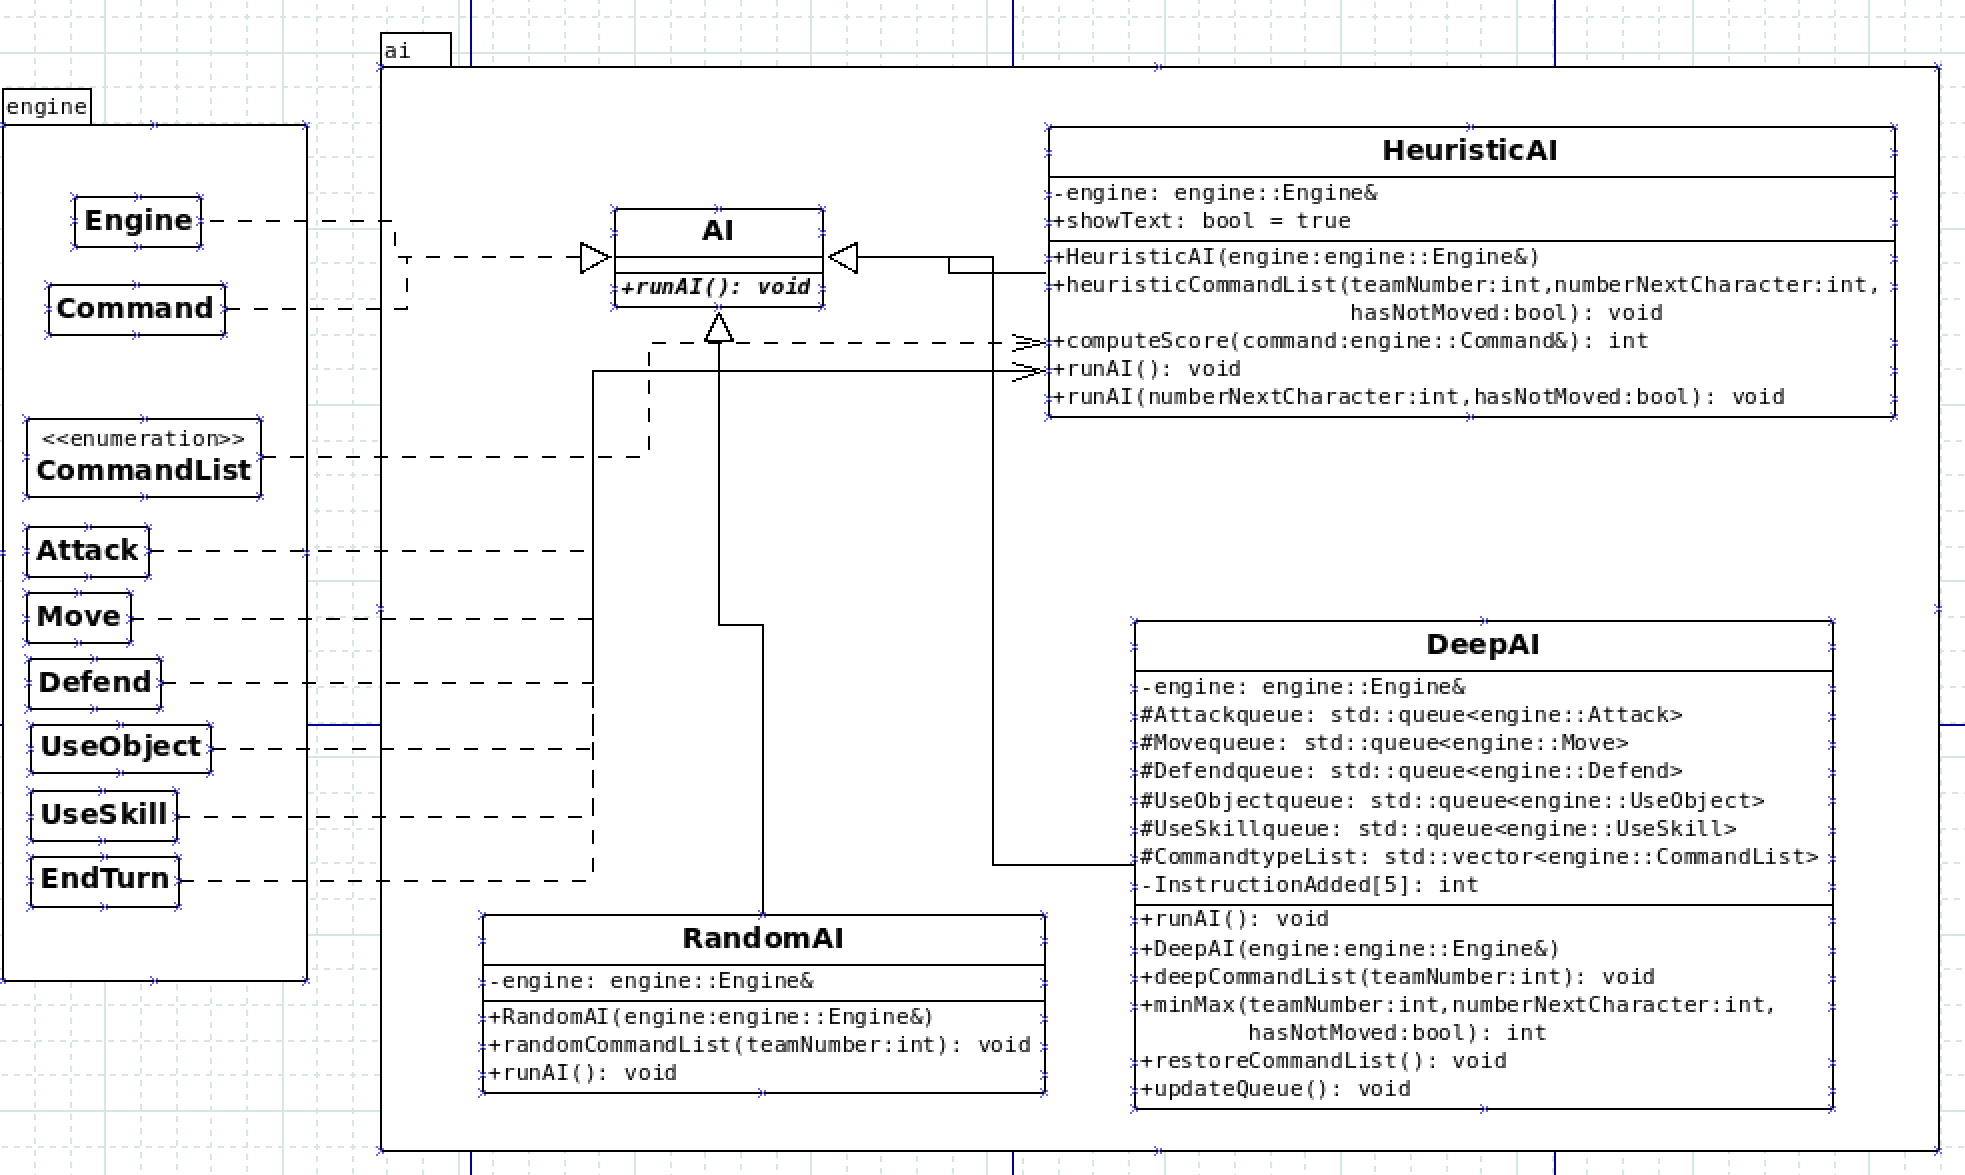
\includegraphics[width=\linewidth]{images/deep_ai_dia.png}
\centering
\caption{Aperçu de ai.dia avec HeuristicAI et DeepAI}
\label{fig:img3}
\end{figure}
\newpage


\newpage

 \nocite{*}
%choix du style de la biblio
\bibliographystyle{plain}
%inclusion de la biblio
\bibliography{bibliographie}
%voir wiki pour plus d'information sur la syntaxe des entrées d'une bibliographie

\end{document}